\documentclass{article}

\usepackage{tikz}
\usetikzlibrary{automata, positioning}
\begin{document}
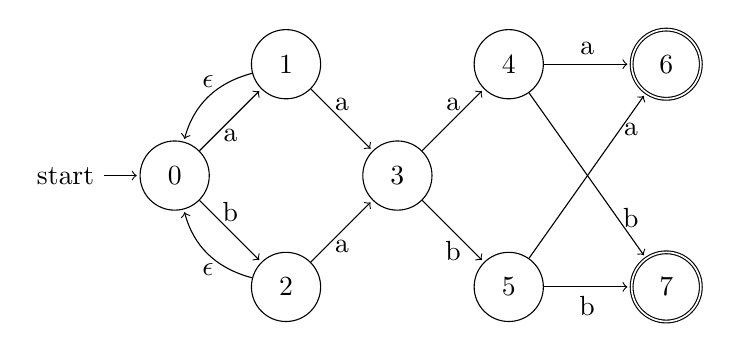
\begin{tikzpicture}[shorten >= 1pt, node distance = 2cm, on grid, auto]
  \node[state, initial] (0) {0};
  \node[state] (1) [above right=of 0] {1};
  \node[state] (2) [below right=of 0] {2};
  \node[state] (3) [below right=of 1] {3};
  \node[state] (4) [above right=of 3] {4};
  \node[state] (5) [below right=of 3] {5};
  \node[state, accepting] (6) [right=of 4] {6};
  \node[state, accepting] (7) [right=of 5] {7};
  \path[->]
    (0) edge node [below] {a} (1)
        edge node [above] {b} (2)
    (1) edge node [above] {a} (3)
        edge [bend right] node [above] {$\epsilon$} (0)
    (2) edge node [below] {a} (3)
        edge [bend left] node [below] {$\epsilon$} (0)
    (3) edge node [above] {a} (4)
        edge node [below] {b} (5)
    (4) edge node [above] {a} (6)
        edge node [above, very near end] {b} (7)
    (5) edge node [below, very near end] {a} (6)
        edge node [below] {b} (7);
\end{tikzpicture}
\end{document}
